\subsection{问题一的模型的建立和求解}

\subsubsection{具体分析}

针对问题一，本问属于\textbf{综合评价与回归建模}类问题，需要完成三项递进任务：一是对 22 个质量指标进行预处理并建立综合评价模型，给出样本级、语料级与领域级质量评分 $Q$；二是定义并消解不同质量指标之间的冲突；三是建立 17 域配比 $\bm p$ 与交叉熵损失之间的定量关系并验证。本问综合采用指标方向统一、极差归一化与熵权法进行质量评价，采用成对标准化得分差与 Kendall 协同系数进行冲突检验与消解，采用岭正则线性混合回归（Ridge Mixture Regression）刻画配比—损失关系\cite{xie2023doremi}。

首先对质量信号数据进行清洗，将 22 个质量指标（含 8 个多维列表型指标）统一为“越高越好”的方向并压缩为标量，建立综合评价模型得到质量评分 $Q$；接着定义“冲突”为两指标标准化得分之差超过阈值的情形，用 Kendall 协同系数检验指标一致性并给出消解规则；然后利用训练配方表与损失表建立配比 $p_k$ 到各域损失 $L_d$ 的线性混合回归模型，并以岭正则处理成分数据的闭合效应与未测量域；最后在 1M、60M、1B 三套检验集上验证，并利用 10B、70B 外推表讨论跨尺度外推的稳健性。

\subsubsection{模型准备}

\textbf{1.数据预处理}

附件 A 的配方表（A4）以 17 个 The Pile 子领域的训练配比 $p_k$（分量非负且和为 1）为特征\cite{gao2020pile}，损失表（A5）以 13 个验证域的交叉熵损失为响应，二者通过 index 列一一对应。17 个训练域中 nih\_exporter、enron\_emails、europarl、philpapers 仅有配比列而无对应损失列，本文保留其配比分量但在系数解释时标注为“间接影响域”。质量信号数据（A1--A3）含 22 个质量指标，其方向并不统一，须先逐指标统一为“越高越好”。设第 $j$ 个指标的原始取值为 $x_j$，对正向指标直接做极差归一化，对负向指标先取补再归一化，对“长度型”指标（过长过短均不佳）转为中心接近度：
\begin{equation}
    x'_j = \begin{cases}
        \dfrac{x_j-\min x_j}{\max x_j-\min x_j}, & \text{正向指标}\\[6pt]
        \dfrac{\max x_j-x_j}{\max x_j-\min x_j}, & \text{负向指标}\\[6pt]
        \exp\!\left(-\dfrac{|\ln(1+x_j)-m_j|}{2.5\,\text{MAD}_j}\right), & \text{长度型指标}
    \end{cases}
\end{equation}
其中 $m_j$ 与 $\text{MAD}_j$ 为对数尺度的中位数与中位绝对偏差；$x'_j\in[0,1]$ 且统一为“越高越好”。22 个指标的方向判定与语义说明见表\ref{tab:p1_dir}，其中 8 个多维列表型指标（原始为有序类别 logits）先按 softmax 概率取归一化期望级别压缩为标量，再参与归一化。

\begin{longtable}{>{\raggedright\arraybackslash}p{0.30\textwidth}>{\centering\arraybackslash}p{0.12\textwidth}>{\raggedright\arraybackslash}p{0.20\textwidth}>{\centering\arraybackslash}p{0.10\textwidth}>{\centering\arraybackslash}p{0.12\textwidth}}
  \caption{22 个质量指标的方向判定与熵权}
  \label{tab:p1_dir} \\
  \toprule
  指标 & 类型 & 语义（方向依据） & 方向 & 熵权 $w_j$ \\
  \midrule
  \endfirsthead
  \caption{22 个质量指标的方向判定与熵权（续）} \\
  \toprule
  指标 & 类型 & 语义（方向依据） & 方向 & 熵权 $w_j$ \\
  \midrule
  \endhead
  \bottomrule
  \endfoot
  fineweb\_edu & 列表(1) & 教育价值 & 正向 & 0.0437 \\
  fluency\_en & 列表(2) & 英语流畅度（第 1 类=流畅，已核验） & 正向 & 0.0682 \\
  modernbert\_cleanliness & 列表(6) & 文本洁净度 & 正向 & 0.1434 \\
  modernbert\_readability & 列表(6) & 可读性 & 正向 & 0.0567 \\
  modernbert\_reasoning & 列表(6) & 推理性 & 正向 & \textbf{0.1517} \\
  modernbert\_professionalism & 列表(6) & 专业性 & 正向 & 0.0396 \\
  dsir\_books & 标量 & 书籍域重要性权重 & 正向 & 0.0081 \\
  dsir\_wiki & 标量 & 维基域重要性权重 & 正向 & 0.0081 \\
  dsir\_math & 标量 & 数学域重要性权重 & 正向 & 0.0086 \\
  qurater & 列表(4) & 教育质量评级（4 项取均值） & 正向 & 0.0492 \\
  ad\_en & 列表(2) & 广告含量（\textbf{第 1 类=“无广告”，正向}；依据：原文抽查） & 正向 & 0.0072 \\
  rps\_doc\_word\_count & 标量 & 文档词数 & 长度型 & 0.0516 \\
  rps\_doc\_num\_sentences & 标量 & 文档句数 & 长度型 & 0.0523 \\
  rps\_doc\_unigram\_entropy & 标量 & 一元词熵（多样性） & 正向 & 0.0347 \\
  rps\_doc\_frac\_unique\_words & 标量 & 唯一词占比 & 正向 & 0.0538 \\
  rps\_doc\_frac\_no\_alph\_words & 标量 & 非字母字符占比 & 负向 & 0.0287 \\
  rps\_doc\_frac\_chars\_top\_2gram & 标量 & 字符 2-gram 重复度 & 负向 & 0.0130 \\
  rps\_doc\_frac\_chars\_top\_3gram & 标量 & 字符 3-gram 重复度 & 负向 & 0.0119 \\
  rps\_lines\_uppercase\_letter\_fraction & 标量 & 大写字母行占比 & 负向 & 0.0316 \\
  rps\_lines\_ending\_with\_terminal\_punctution\_mark & 标量 & 终止标点结尾行占比 & 正向 & 0.0880 \\
  rps\_lines\_numerical\_chars\_fraction & 标量 & 含数字行占比 & 负向 & 0.0125 \\
  rps\_doc\_mean\_word\_length & 标量 & 平均词长 & 长度型 & 0.0373 \\
\end{longtable}

样本级质量评分由各指标加权求和得到，领域级质量 $Q_d$ 为该领域内样本评分的均值：
\begin{equation}
    Q_i = \sum_{j=1}^{22} w_j\, x'_{ij},\qquad Q_d=\frac{1}{n_d}\sum_{i\in\mathcal D_d}Q_i,\qquad \sum_j w_j=1
\end{equation}
其中权重 $w_j$ 由熵权法确定。由表\ref{tab:p1_dir}可见，权重最大的两项是 modernbert\_reasoning（$0.152$）与 modernbert\_cleanliness（$0.143$），即“推理性”与“洁净度”两个信号提供的信息量最多；需要说明的是，熵权法对取值分布的形态较敏感（极端左偏的指标会获得更大权重），因此本文在误差分析中对赋权方案作了敏感性检验（见第\ref{sec:check}节）。

质量信号存在少量字段级缺失，本文流式读取时逐字段审计，结果见表\ref{tab:p1_missing}，并按该指标中位数填充，不把缺失当作高质量或低质量。

\begin{longtable}{>{\raggedright\arraybackslash}p{0.44\textwidth}>{\centering\arraybackslash}p{0.16\textwidth}>{\raggedright\arraybackslash}p{0.36\textwidth}}
  \caption{质量信号的字段级缺失审计（A1--A3 全量 272{,}505 条）}
  \label{tab:p1_missing} \\
  \toprule
  指标 & 缺失记录数 & 形态 \\
  \midrule
  \endfirsthead
  \caption{质量信号的字段级缺失审计（续）} \\
  \toprule
  指标 & 缺失记录数 & 形态 \\
  \midrule
  \endhead
  \bottomrule
  \endfoot
  modernbert\_reasoning & 13 & 整行 6 维取值均为 NaN \\
  modernbert\_professionalism & 6 & 整行 6 维取值均为 NaN \\
  其余 20 个指标 & 0 & 无缺失 \\
\end{longtable}

\textbf{2.算法选择}

本问涉及质量评价（指标聚合）、冲突分析（一致性检验）与配比建模（回归）三类任务，需在候选算法中择优。质量聚合比较熵权法、主成分分析（PCA）第一主成分与等权平均；冲突分析以成对标准化得分差为主、Kendall 协同系数为辅；配比建模比较普通最小二乘、岭回归与随机森林。质量聚合的三种方案对比如表\ref{tab:algo1}所示。

\begin{longtable}{>{\centering\arraybackslash}p{0.20\textwidth}>{\centering\arraybackslash}p{0.16\textwidth}>{\centering\arraybackslash}p{0.20\textwidth}>{\raggedright\arraybackslash}p{0.36\textwidth}}
  \caption{问题一赋权方案对比（样本级相关性与域级排序一致性）}
  \label{tab:algo1} \\
  \toprule
  方案 & 得分均值 & 与熵权法相关性 & 域级 Spearman 排序一致性（对熵权法） \\
  \midrule
  \endfirsthead
  \caption{问题一赋权方案对比（续）} \\
  \toprule
  方案 & 得分均值 & 与熵权法相关性 & 域级 Spearman 排序一致性（对熵权法） \\
  \midrule
  \endhead
  \bottomrule
  \endfoot
  熵权法 & 0.495 & 1.000 & 1.000 \\
  等权平均 & 0.639 & 0.854 & 0.679 \\
  PCA 第一主成分 & 0.520 & 0.881 & 0.679 \\
\end{longtable}

如表\ref{tab:algo1}所示，熵权法能依据指标自身信息量客观赋权、避免主观打分；与等权方案相比，样本级得分相关系数为 $0.854$、域级排序一致性为 $0.679$，说明主体格局稳定但并非完全一致——改用等权后领域排序会发生变化，故本文在误差分析中把赋权方案列入灵敏度检验。PCA 方案虽降维去相关，但主成分含义难以解释，受篇幅限制不作备选。配比建模中 17 域配比满足单纯形约束（和为 1）而天然存在共线性，岭回归通过 $L_2$ 正则化能稳定估计且外推可解释，故采用岭正则线性混合回归。冲突分析方面，Kendall 协同系数刻画的是“指标作为评价者”的整体一致性，而问题要求的是“对同一文本给出显著不一致评价”的样本级冲突，二者互补，故同时报告。

\subsubsection{模型建立}

\textbf{步骤1：质量评价模型}

设 $m$ 条质量信号样本、22 个指标经方向统一与归一化后构成矩阵 $\bm X=(x'_{ij})$。第 $j$ 个指标的信息熵与熵权为：
\begin{equation}
    e_j = -\frac{1}{\ln m}\sum_{i=1}^{m} f_{ij}\ln f_{ij},\qquad f_{ij}=\frac{x'_{ij}+\varepsilon}{\sum_i (x'_{ij}+\varepsilon)},\qquad
    w_j = \frac{1-e_j}{\sum_{j=1}^{22}(1-e_j)}
\end{equation}
为与附件 B 的损失数据耦合，本问同时给出“结果导向”的领域质量代理指标：以各验证域在平均配方下的观测损失表征领域内在难度并映射为质量：
\begin{equation}
    Q_d^{(\text{loss})}=1-\frac{\bar L_d-\min_d \bar L_d}{\max_d \bar L_d-\min_d \bar L_d}
\end{equation}
其中 $\bar L_d$ 为领域 $d$ 的平均交叉熵损失。该代理指标仅在 13 个可测损失域上有定义，与 A1--A3 的 7 个质量域并非同一分类体系，二者的关联由 A16 映射表建立、并在模型求解中作一致性检验。

\textbf{步骤2：质量冲突消解模型}

当两个质量指标对同一文本给出显著不一致的评价时即产生冲突。以方向统一后的标准化得分为基础，定义第 $i$ 样本在指标 $j$ 与 $k$ 上的冲突指示：
\begin{equation}
    \delta_i(j,k) = \left| z_{ij} - z_{ik} \right|,\qquad z_{ij}=\frac{x'_{ij}-\mu_j}{\sigma_j},\qquad
    \mathbf 1\{\delta_i(j,k)>\tau\}
\end{equation}
取阈值 $\tau=1.5$；全样本冲突率为
\begin{equation}
    \rho_c = \frac{1}{m\binom{22}{2}}\sum_{i=1}^{m}\sum_{j<k}\mathbf 1\{\delta_i(j,k)>\tau\}
\end{equation}
为给出参照系，本文同时计算“指标独立”基准 $\rho_0=2\Phi(-\tau/\sqrt2)$：若 $\rho_c/\rho_0<1$，说明指标间存在正相关、并非互相矛盾。指标间整体一致性用 Kendall 协同系数检验（22 个指标为评价者、$m$ 条文本为评价对象）：
\begin{equation}
    W = \frac{12\sum_i (R_i-\bar R)^2}{22^2\,(m^3-m)},\qquad R_i=\sum_{j=1}^{22} r_{ij},\qquad
    \chi^2 = 22(m-1)W
\end{equation}
其中 $r_{ij}$ 为第 $i$ 样本在第 $j$ 指标上的秩。消解规则为：若某样本被判为冲突，则以其上“多数指标”的方向（即加权得分 $Q_i$ 相对该样本所在域中位数的偏离方向）作为该样本的最终质量裁决，并在报告中保留冲突标记以供下游剔除或降权。

\textbf{步骤3：领域配比建模（线性混合回归）}

设训练配方矩阵 $\bm P\in[0,1]^{n\times 17}$（行和为 1），损失矩阵 $\bm L\in\mathbb R^{n\times 13}$。建立各验证域损失对配比的线性混合模型：
\begin{equation}
    L_{d}(\bm p) = \sum_{k=1}^{17} a_{dk}\, p_k + b_d,\qquad d=1,\dots,13
    \qquad\Longleftrightarrow\qquad
    \hat{\bm L} = \bm P \bm A + \bm 1 \bm b^{\top}
\end{equation}
由于 $\bm P$ 各行和为 1，回归存在闭合不可辨识性，采用岭正则估计系数矩阵 $\bm A\in\mathbb R^{17\times 13}$ 与截距 $\bm b$：
\begin{equation}
    \min_{\bm A,\bm b}\ \left\|\bm L-\bm P\bm A-\bm 1\bm b^{\top}\right\|_F^2 + \lambda\left\|\bm A\right\|_F^2,
    \qquad
    \begin{bmatrix}\bm A\\ \bm b^{\top}\end{bmatrix}
    = \left(\tilde{\bm P}^{\top}\tilde{\bm P}+\lambda \bm D\right)^{-1}\tilde{\bm P}^{\top}\bm L
\end{equation}
其中 $\tilde{\bm P}=[\bm P,\ \bm 1]$，$\bm D=\mathrm{diag}(1,\dots,1,0)$（不惩罚截距），$\lambda=10^{-3}$。

\textbf{步骤4：质量信息的引入方式与检验}

问题一要求论证“是否以及如何引入质量评分 $Q$”。本文构造混合质量指数 $\bar Q(\bm p)=\sum_k p_k Q_k$（$Q_k$ 由 A16 映射得到：direct/near\_direct 域直接取用 A1--A3 域级质量，inferred 域取全局均值），并做增量回归检验：
\begin{equation}
    \hat{\bm L} = \bm P \bm A + \bm 1 \bm b^{\top} + \bm 1\, c^{\top}\bar Q(\bm p)
\end{equation}
若质量项带来的 $R^2$ 增量可忽略，则说明线性配比已吸收质量信息，此时不宜重复引入以免共线；质量评分转而作为独立资源交由问题二、三使用。

\textbf{步骤5：最优配比与稳健推荐}

在系数矩阵 $\bm A$ 基础上，固定未测量域配比于参考值，优化 13 个可测域的配比使加权平均损失最小：
\begin{equation}
    \min_{\bm p\in\Delta_{17}}\ \sum_{d\in\mathcal M} w_d\left(\sum_k a_{dk}p_k+b_d\right),
    \qquad \Delta_{17}=\left\{\bm p:\ p_k\ge0,\ \textstyle\sum_k p_k=1\right\}
\end{equation}
为给出可落地的稳健方案，进一步限制各域配比不超过参考配比的 2.5 倍，得到有界推荐配比。

\subsubsection{模型求解}

基于上述模型，利用附件 A 的质量信号（A1--A3）与配方/损失数据（A4--A15）进行求解，共处理全量质量记录 $272{,}505$ 条（A1 抽样集 $51{,}230$ 条、A2+A3 扩展集 $221{,}275$ 条）。

\textbf{1.质量评分与冲突分析}

质量域的领域级评分如图\ref{fig:p1_quality_full}所示，A1 抽样集与扩展集的对照结果如表\ref{tab:p1_qa}所示。

\begin{figure}[ht]
  \centering
  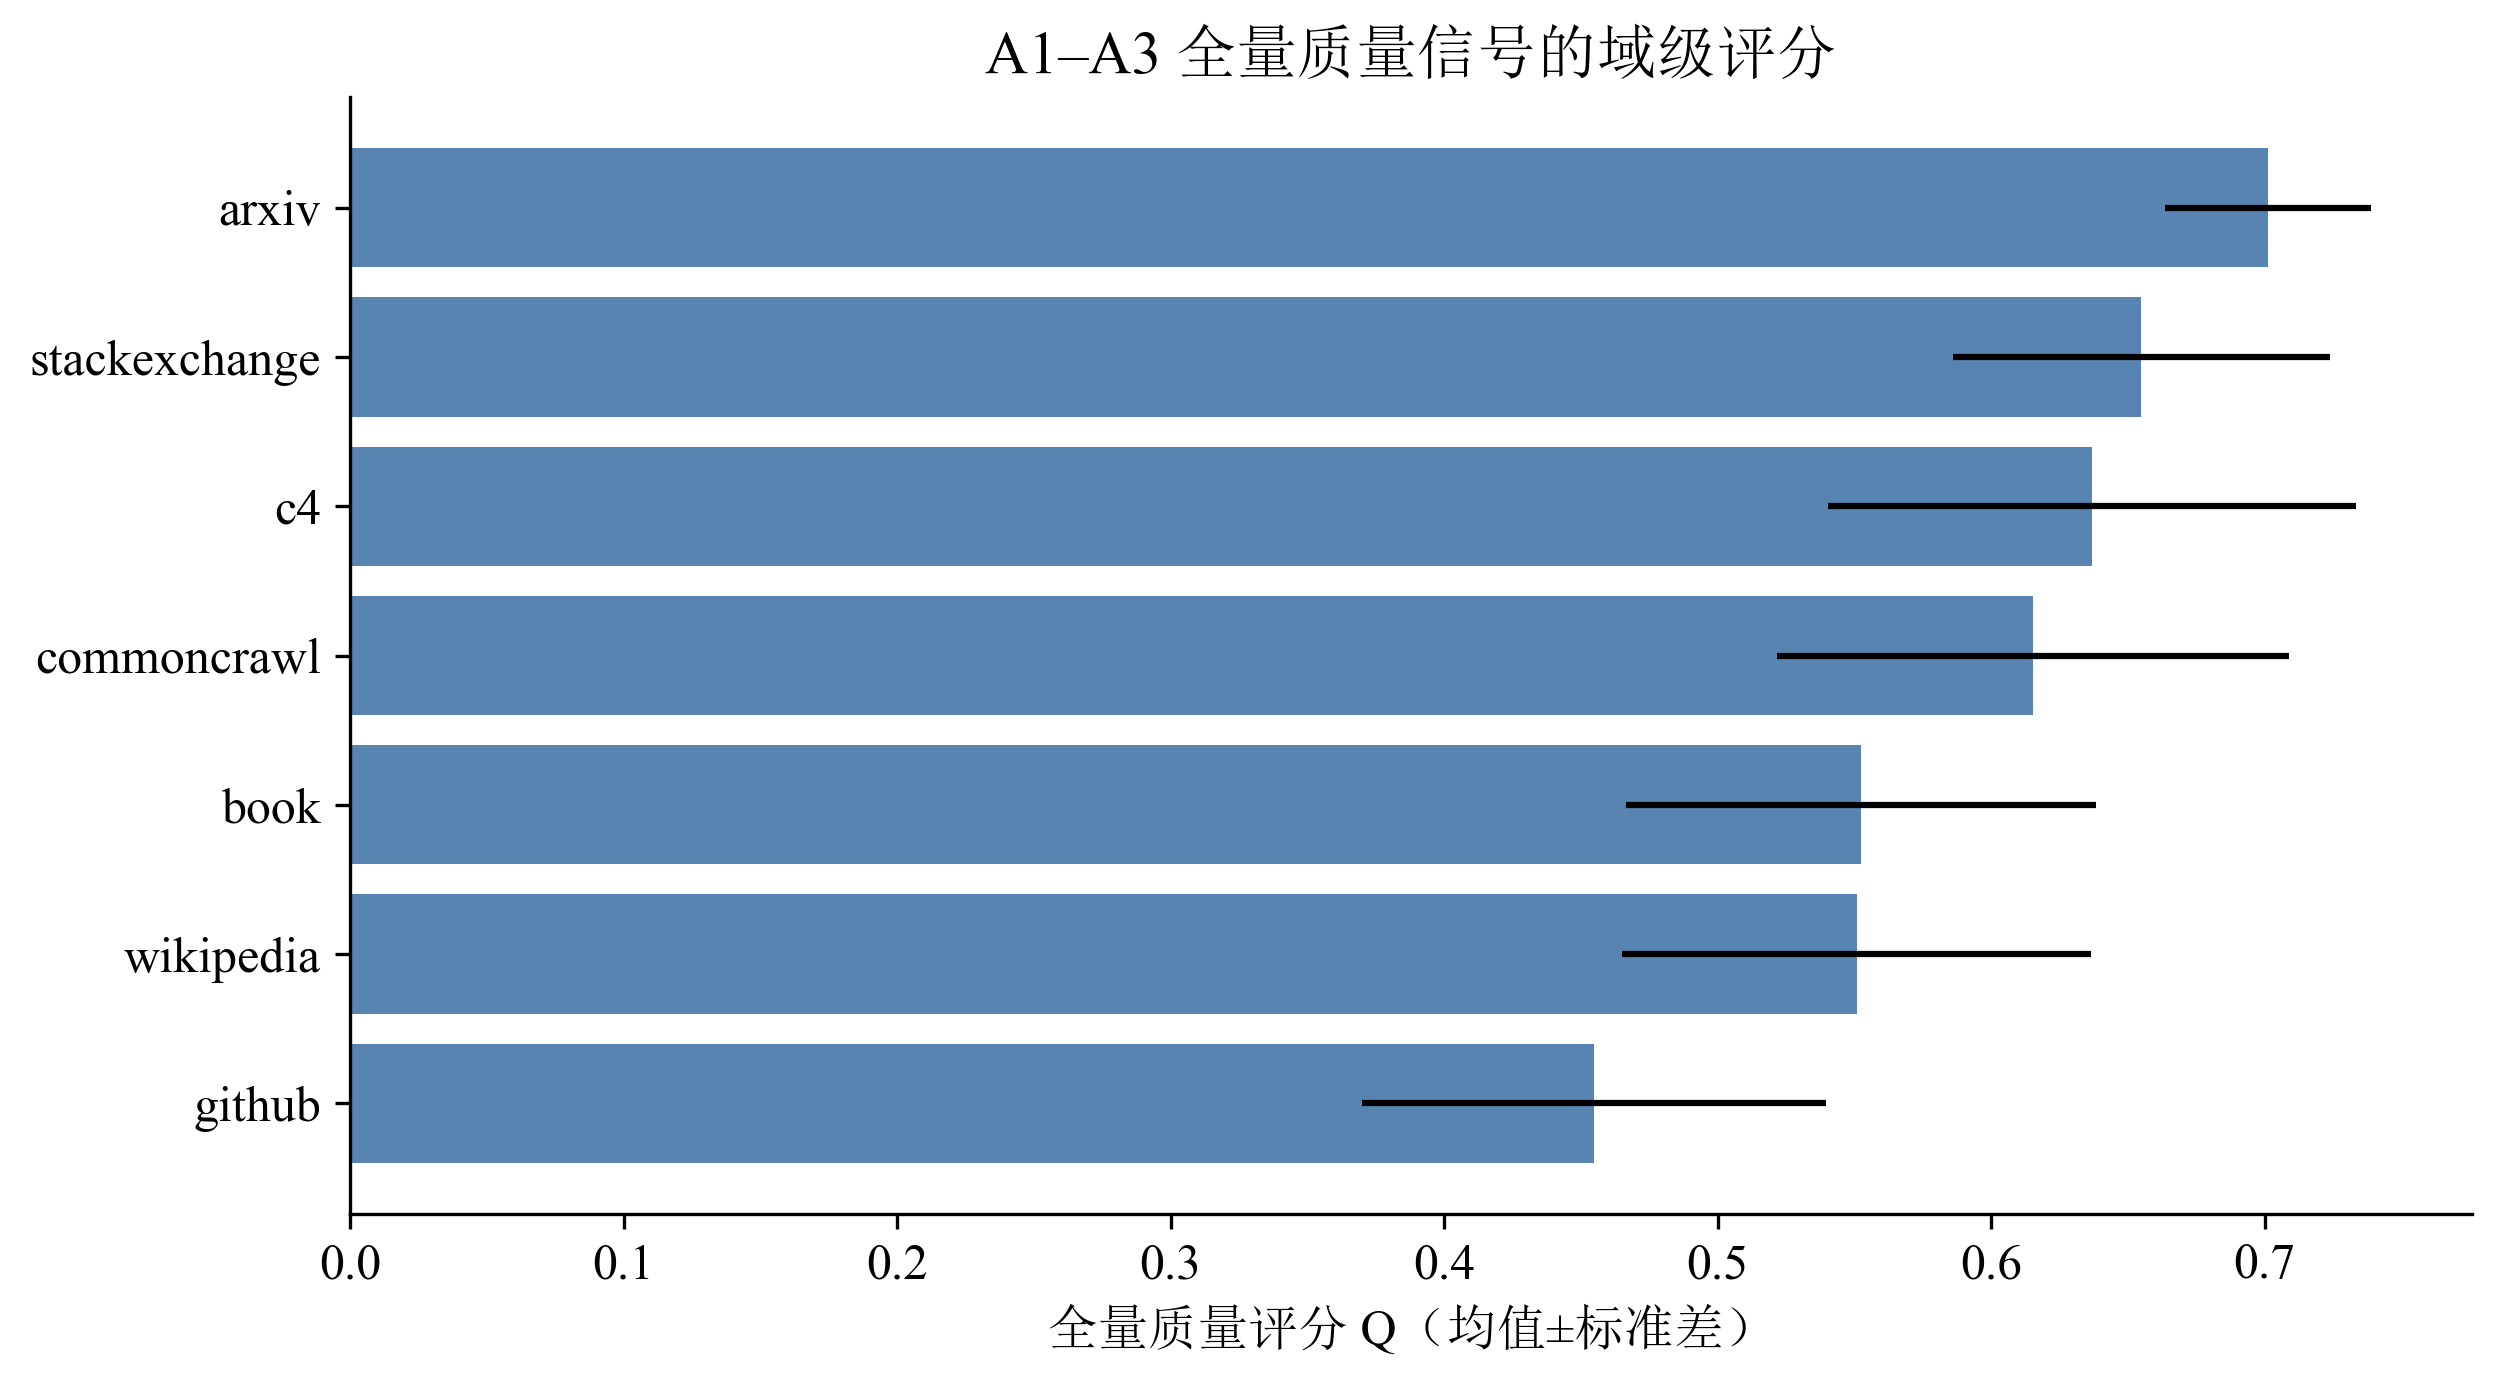
\includegraphics[width=0.62\textwidth]{求解/问题一/图片/图0_A1-A3全量质量评分.png}
  \caption{A1--A3 全量质量信号的领域级评分（均值±标准差）}
  \label{fig:p1_quality_full}
\end{figure}

\begin{longtable}{>{\centering\arraybackslash}p{0.20\textwidth}>{\centering\arraybackslash}p{0.16\textwidth}>{\centering\arraybackslash}p{0.16\textwidth}>{\centering\arraybackslash}p{0.16\textwidth}>{\raggedright\arraybackslash}p{0.24\textwidth}}
  \caption{抽样集 A1 与扩展集 A2/A3 的域级质量对照}
  \label{tab:p1_qa} \\
  \toprule
  质量域 & $Q$（A1） & $Q$（扩展集） & 差值 & 对应配方域 \\
  \midrule
  \endfirsthead
  \caption{抽样集 A1 与扩展集 A2/A3 的域级质量对照（续）} \\
  \toprule
  质量域 & $Q$（A1） & $Q$（扩展集） & 差值 & 对应配方域 \\
  \midrule
  \endhead
  \bottomrule
  \endfoot
  arxiv & 0.7031 & 0.7011 & $+0.0021$ & arxiv \\
  stackexchange & 0.6549 & — & — & stackexchange \\
  c4 & 0.6368 & — & — & （配方侧无同名列） \\
  commoncrawl & 0.6153 & — & — & pile\_cc \\
  book & 0.5524 & — & — & gutenberg\_pg\_19 \\
  wikipedia & 0.5509 & — & — & wikipedia\_en \\
  github & 0.4553 & 0.4547 & $+0.0006$ & github \\
\end{longtable}

由表\ref{tab:p1_qa}可知，在同时具有抽样与扩展质量信号的两个域上（arxiv、github），两种口径的域级质量差异不超过 $0.002$（arxiv $+0.0021$、github $+0.0006$），说明抽样集对扩展集具有代表性、评分口径可跨集合迁移。全体记录的领域质量排序为 arxiv（0.703）$>$ stackexchange（0.655）$>$ c4（0.637）$>$ commoncrawl（0.615）$>$ book（0.552）$\approx$ wikipedia（0.551）$>$ github（0.455）。需要指出，该排序是 22 个分类器信号的合成结果，其中若干信号（如 rps\_doc\_frac\_unique\_words、rps\_doc\_unigram\_entropy）与文档长度相关，因此“c4/commoncrawl 高于 book/wikipedia”反映的是信号体系的口径，而非对语料价值的终极判断——这一点在使用该评分时须注意。

冲突与一致性检验结果如表\ref{tab:p1_conf}所示，冲突最集中的指标对与熵权分布见图\ref{fig:p1_conf}。

\begin{longtable}{>{\centering\arraybackslash}p{0.18\textwidth}>{\centering\arraybackslash}p{0.13\textwidth}>{\centering\arraybackslash}p{0.13\textwidth}>{\centering\arraybackslash}p{0.13\textwidth}>{\centering\arraybackslash}p{0.14\textwidth}>{\raggedright\arraybackslash}p{0.20\textwidth}}
  \caption{质量冲突与一致性检验结果}
  \label{tab:p1_conf} \\
  \toprule
  数据集 & 样本数 & Kendall $W$ & 冲突率 $\rho_c$ & 独立基准 $\rho_0$ & $\rho_c/\rho_0$ \\
  \midrule
  \endfirsthead
  \caption{质量冲突与一致性检验结果（续）} \\
  \toprule
  数据集 & 样本数 & Kendall $W$ & 冲突率 $\rho_c$ & 独立基准 $\rho_0$ & $\rho_c/\rho_0$ \\
  \midrule
  \endhead
  \bottomrule
  \endfoot
  A1 抽样集 & 51{,}230 & 0.0783 & 0.2252 & 0.2888 & 0.780 \\
  A2+A3 扩展集 & 221{,}275 & 0.0628 & 0.2208 & 0.2888 & 0.764 \\
  全量 & 272{,}505 & 0.0687 & 0.2235 & 0.2888 & 0.774 \\
\end{longtable}

\begin{figure}[ht]
  \centering
  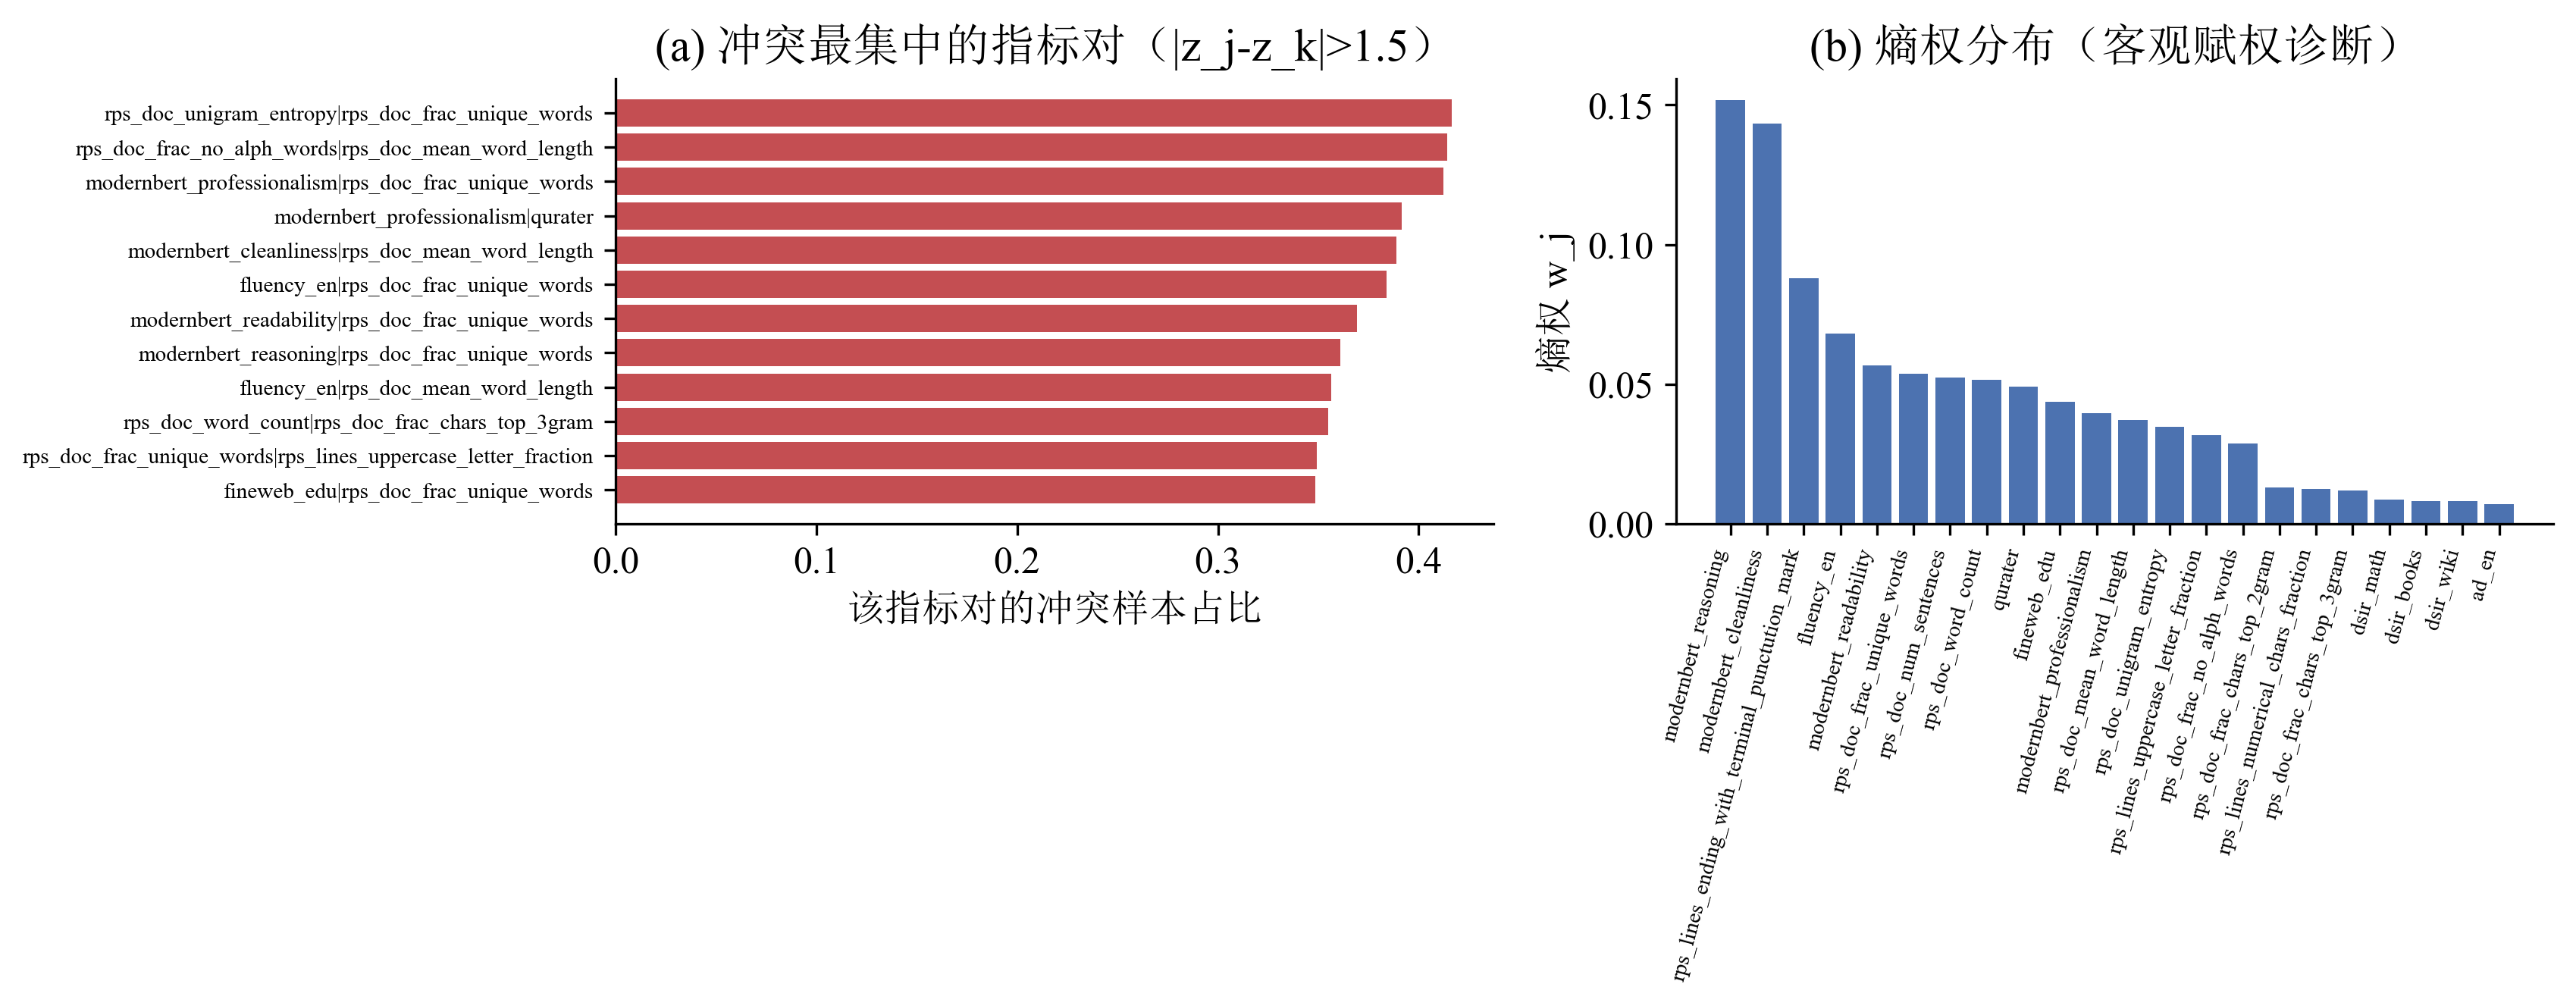
\includegraphics[width=0.92\textwidth]{求解/问题一/图片/图6_冲突与赋权诊断.png}
  \caption{冲突最集中的指标对（左）与熵权分布（右）}
  \label{fig:p1_conf}
\end{figure}

由表\ref{tab:p1_conf}可知：（1）三套数据的冲突率几乎一致（$0.221\sim0.225$），说明冲突结构在抽样集与扩展集上同样成立，A2/A3 的结论可外推至 A1 所代表的总体；（2）Kendall 协同系数为 $0.069$（$\chi^2$ 检验 $p<0.001$，样本量极大故显著性很高），属于“正相关但一致性较弱”的水平，与冲突率 $22.3\%$ 一致，说明“各质量指标完全一致、不存在冲突”的判断并不成立；（3）但冲突率低于指标完全独立时的基准 $28.9\%$（比值 $0.774$），说明指标间确为正相关，冲突主要发生在语义上本就不同的指标之间。冲突成因可归纳为三类：一是度量对象不同（如 rps\_doc\_unigram\_entropy 与 rps\_doc\_frac\_unique\_words 同测“多样性”但量纲不同），二是内容类型差异（如 modernbert\_professionalism 对学术文本与论坛文本的评价尺度不同），三是分布形态差异（如 ad\_en 为二分类概率、在长文档上两极化）。据此本文按“多数指标方向裁决 + 冲突标记保留”的规则消解：冲突样本仍参与领域均值，但以 $Q_i$ 相对域中位数的偏离方向标注其可信度，并在问题二、三中不单独使用冲突样本。

\textbf{2.配比—损失建模与验证}

配方结构与拟合、泛化表现分别如图\ref{fig:p1_structure}与图\ref{fig:p1_r2}所示，预测—实测对比如图\ref{fig:p1_scatter}所示，系数热力图如图\ref{fig:p1_heatmap}所示。

\begin{figure}[ht]
  \centering
  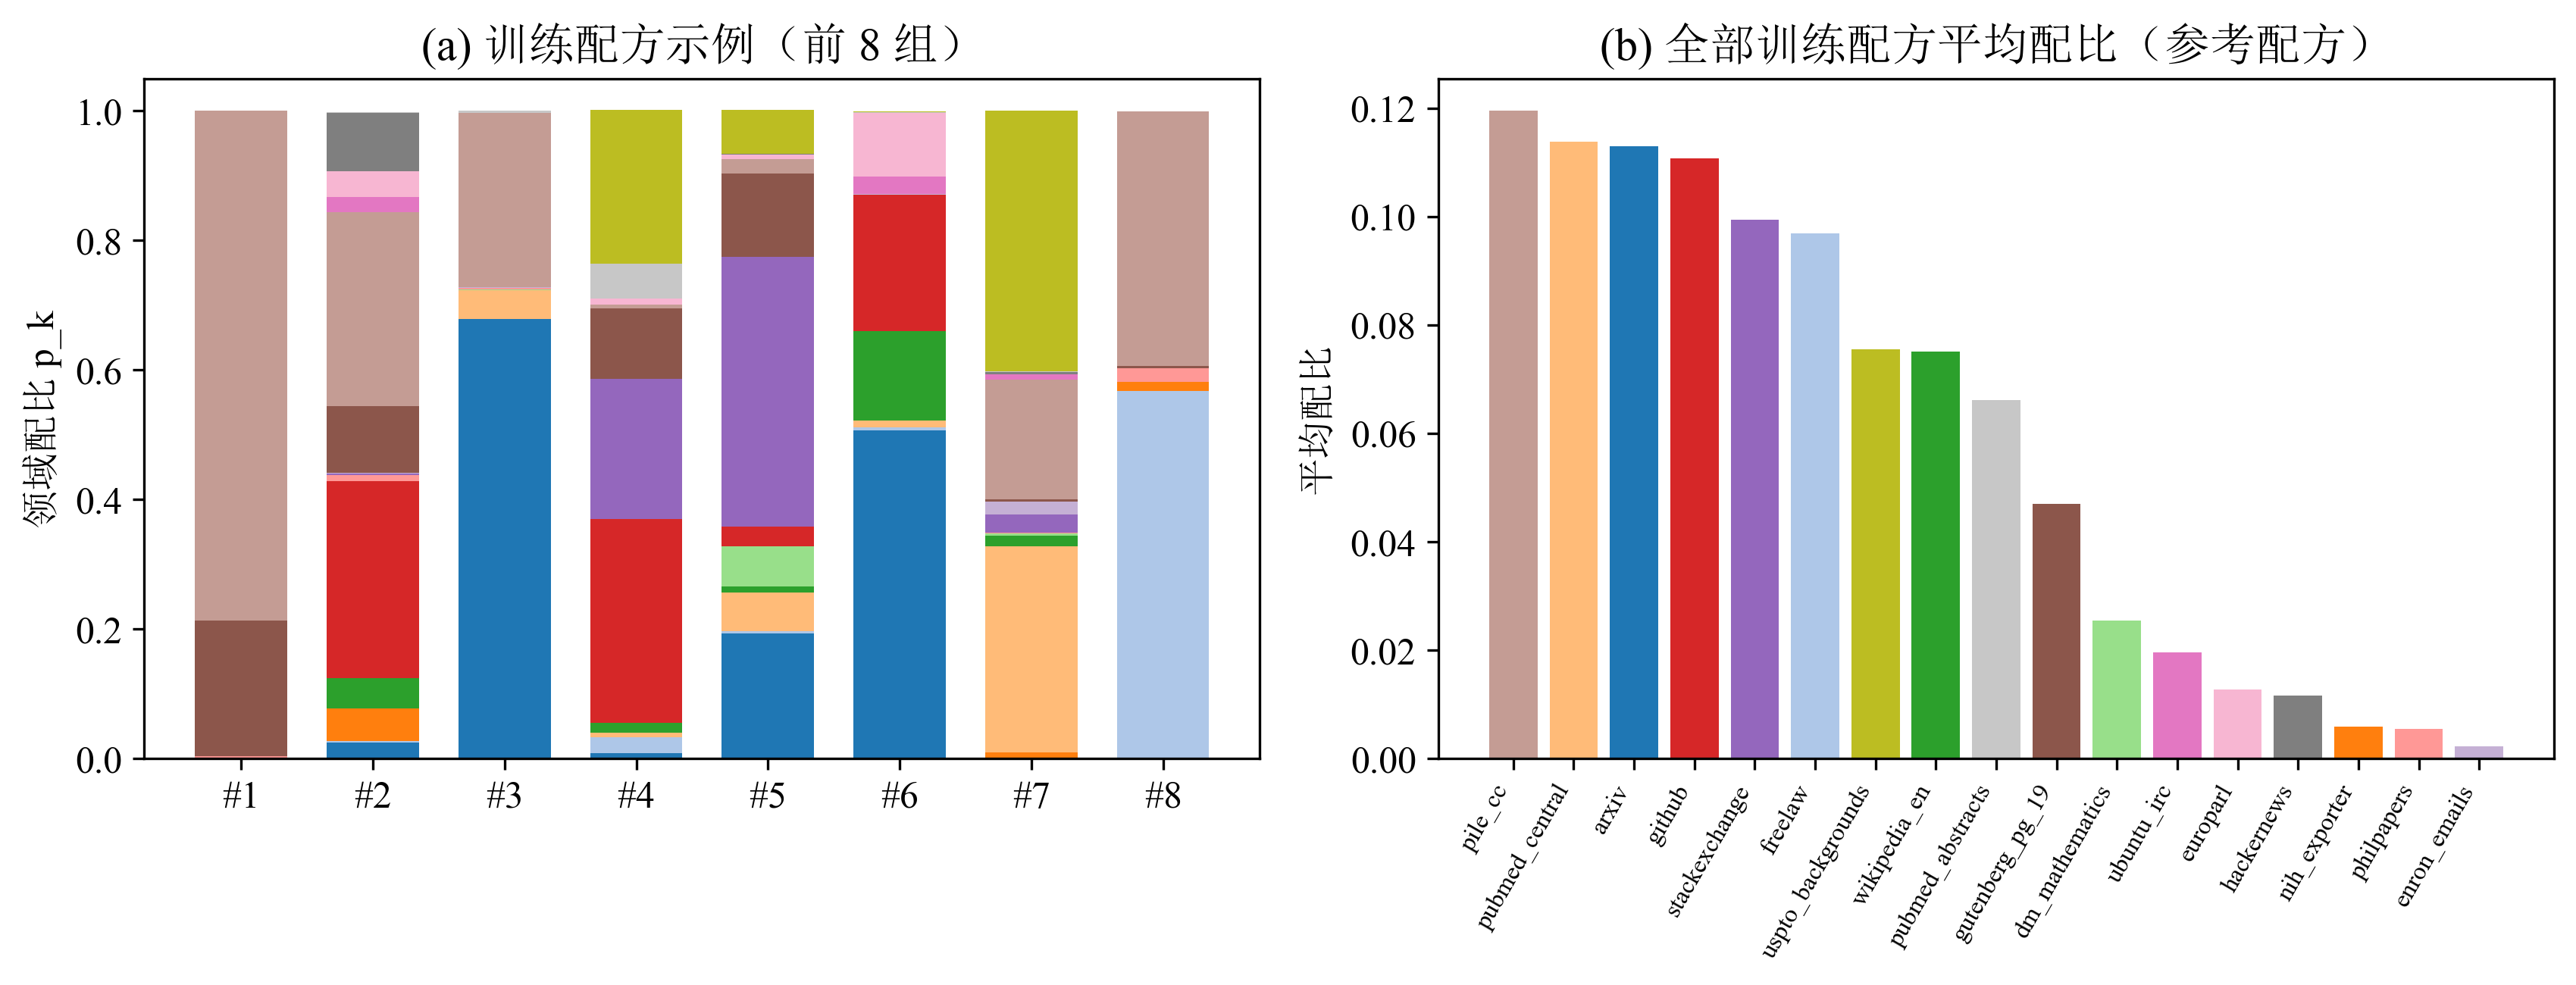
\includegraphics[width=0.92\textwidth]{求解/问题一/图片/图1_训练配比结构.png}
  \caption{训练配方结构（左：前 8 组配方堆叠；右：全部配方平均配比）}
  \label{fig:p1_structure}
\end{figure}

\begin{figure}[ht]
  \centering
  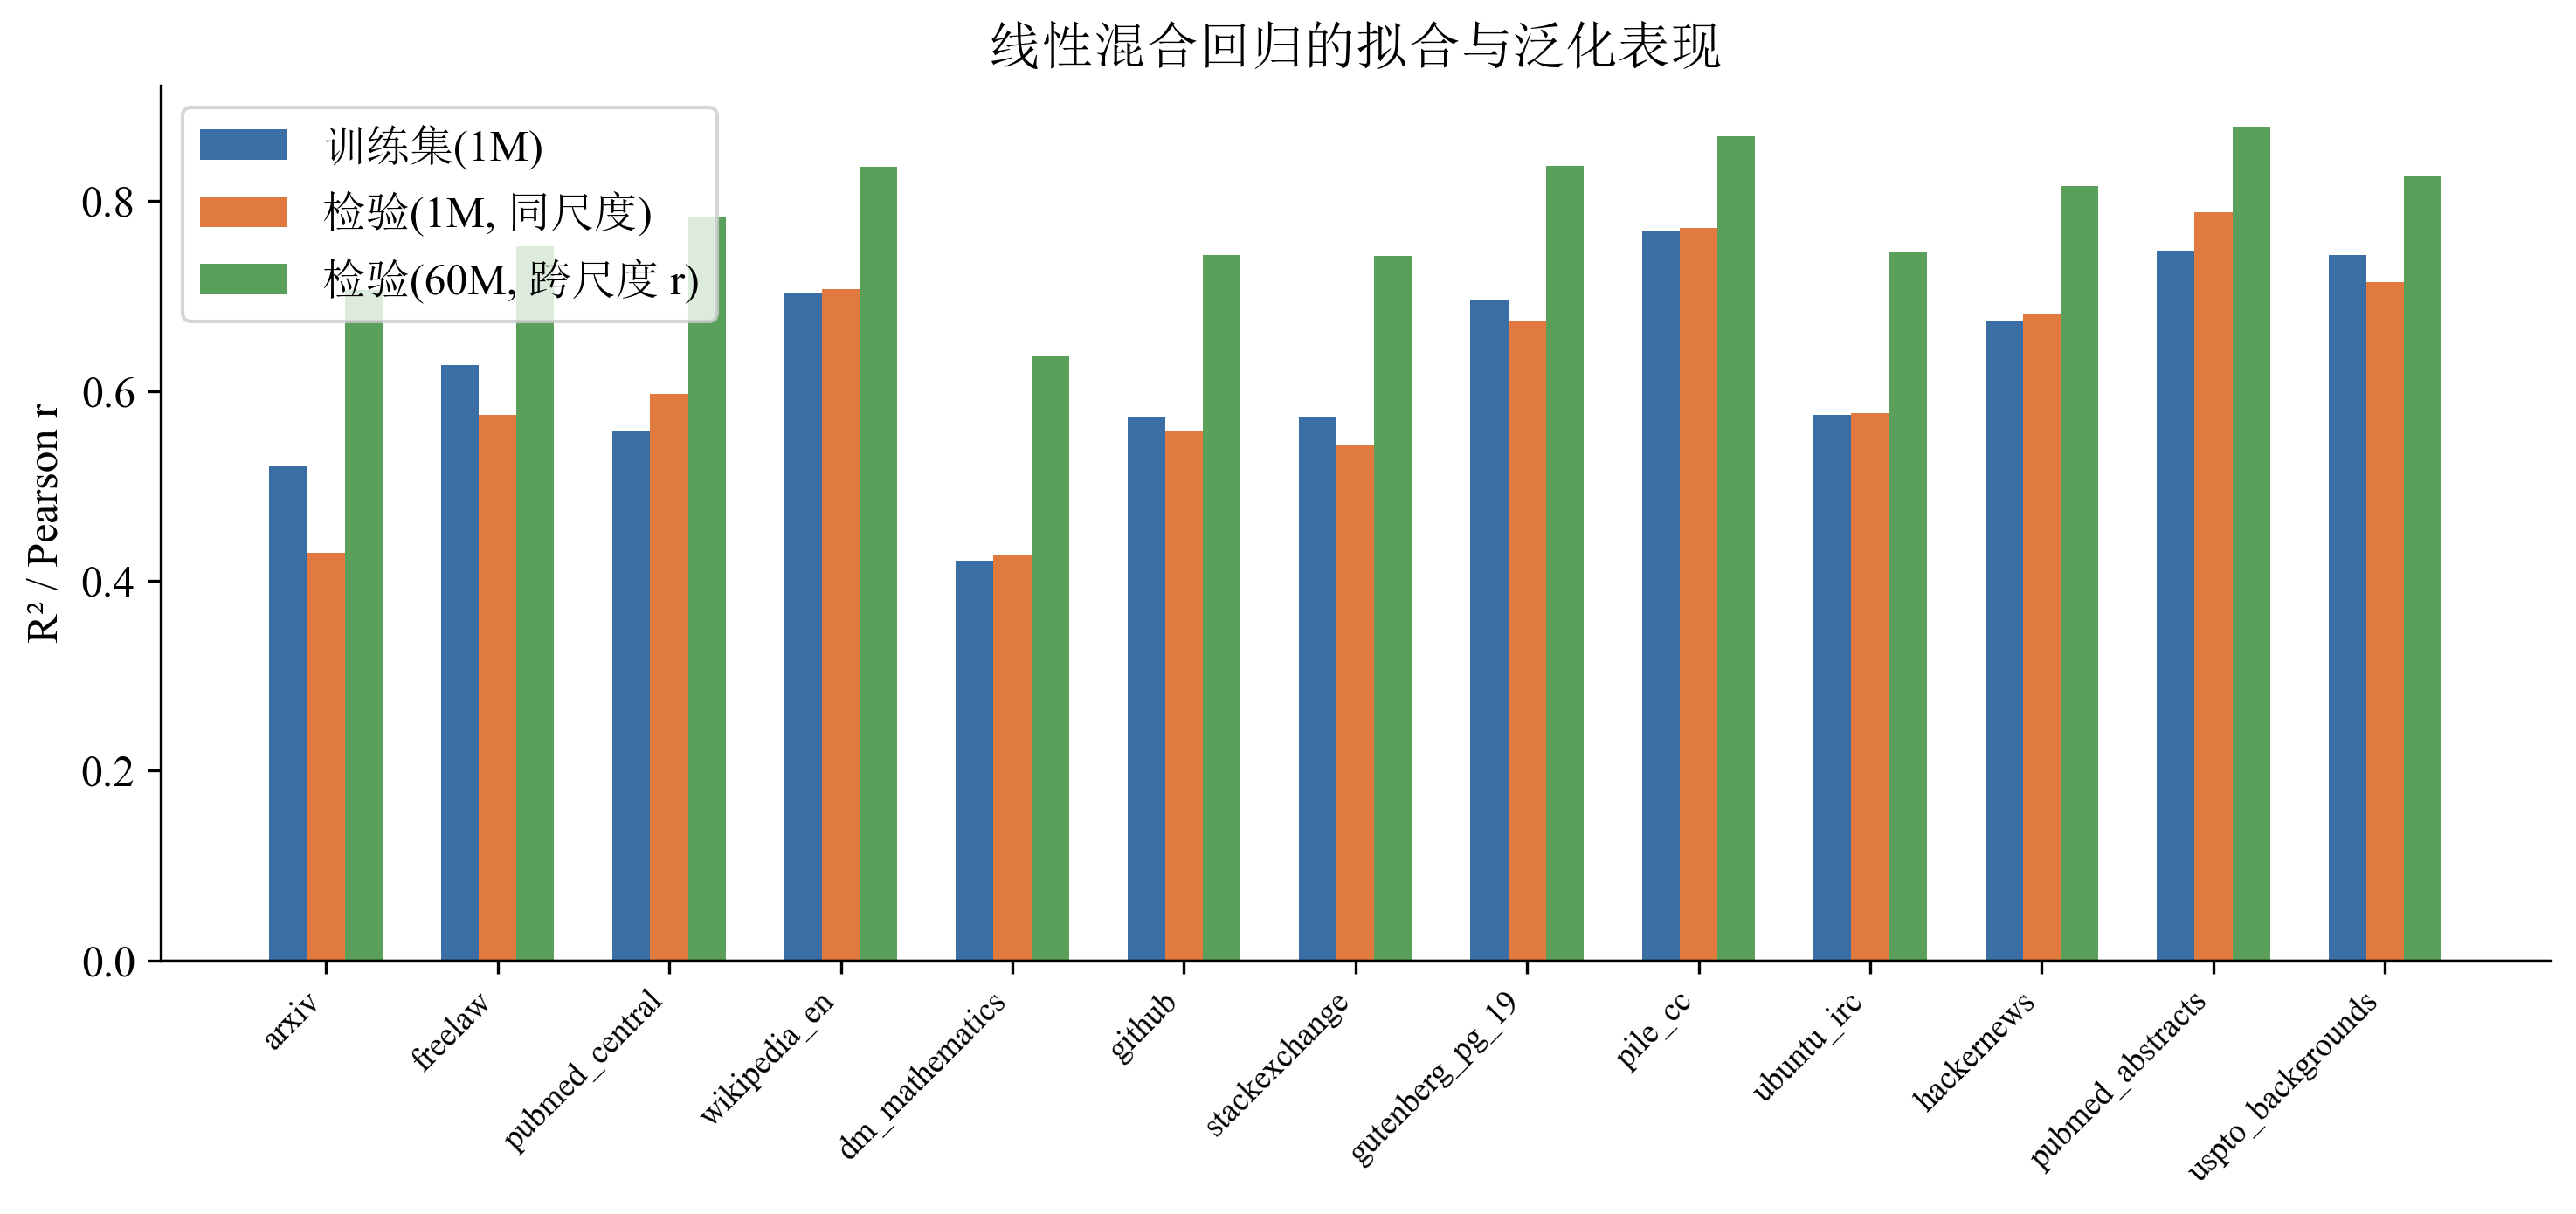
\includegraphics[width=0.72\textwidth]{求解/问题一/图片/图2_线性模型R2.png}
  \caption{线性混合回归的拟合与泛化表现}
  \label{fig:p1_r2}
\end{figure}

\begin{figure}[ht]
  \centering
  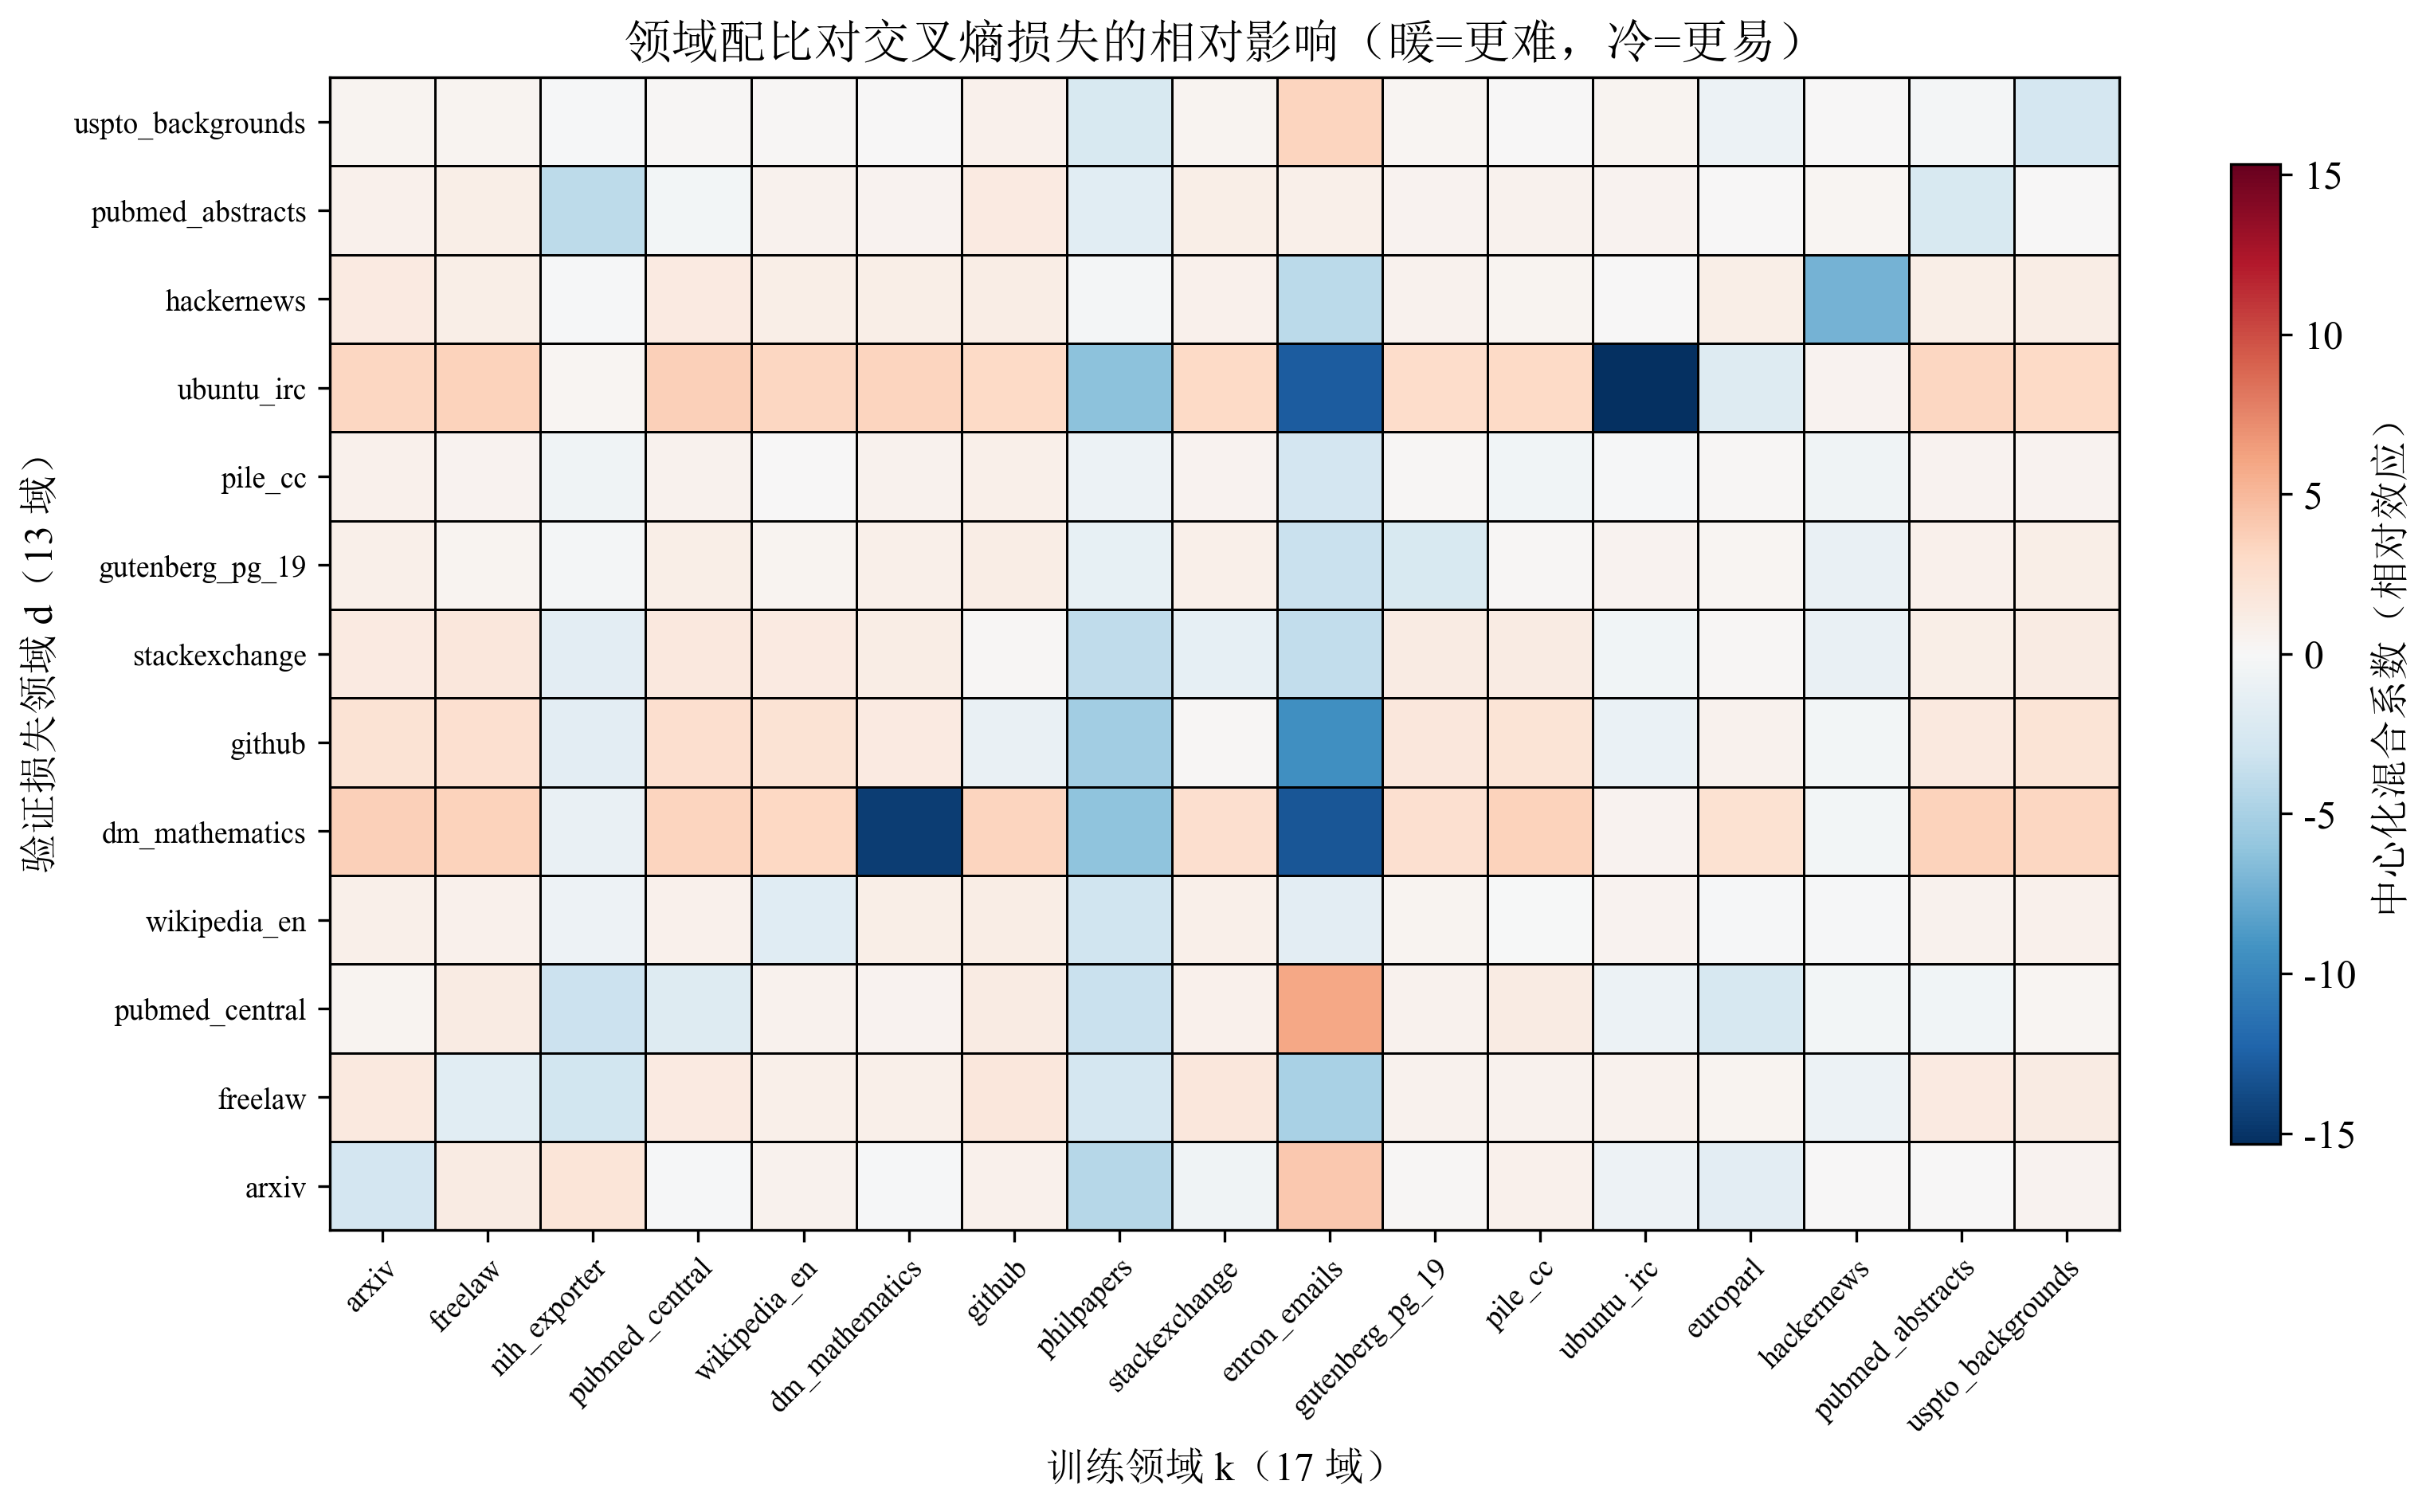
\includegraphics[width=0.78\textwidth]{求解/问题一/图片/图4_混合系数热力图.png}
  \caption{领域配比对交叉熵损失的相对影响热力图}
  \label{fig:p1_heatmap}
\end{figure}

\begin{figure}[ht]
  \centering
  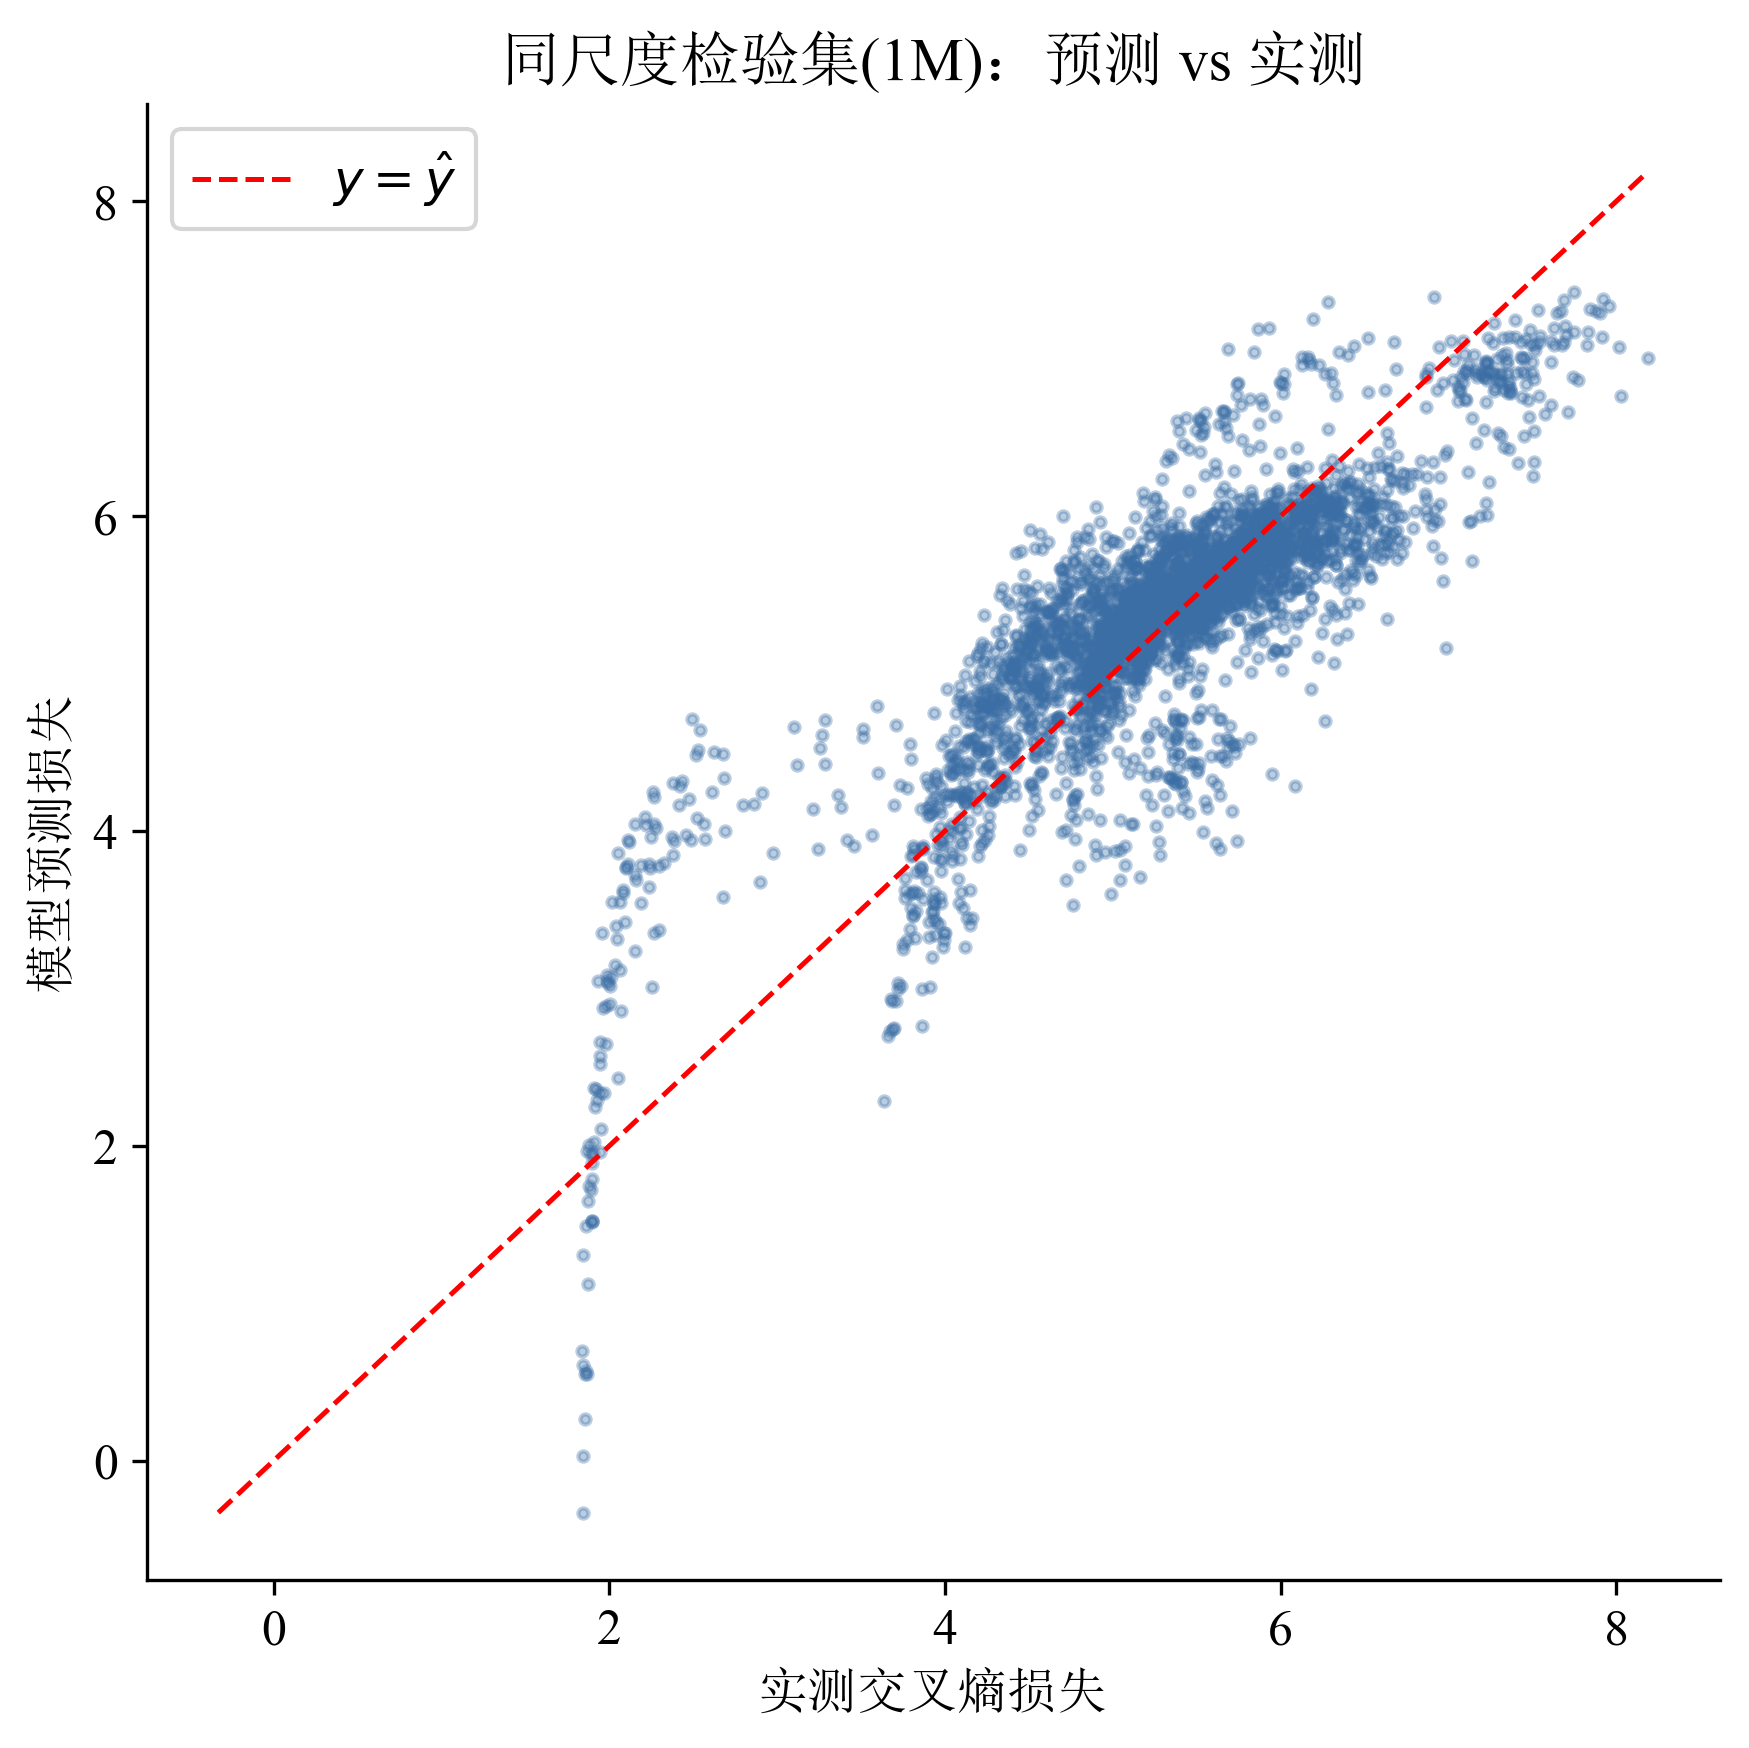
\includegraphics[width=0.58\textwidth]{求解/问题一/图片/图3_预测vs实测.png}
  \caption{同尺度检验集（1M）预测损失与实测损失对比}
  \label{fig:p1_scatter}
\end{figure}

由图\ref{fig:p1_r2}可知，训练集上 13 个损失域的 $R^2$ 位于 $0.42\sim0.77$ 之间、平均 $0.629$；同尺度 1M 检验集平均 $R^2=0.619$，与训练接近，说明模型未明显过拟合。由于不同参数规模下损失水平本身不同（60M 与 1M 的损失比约 $0.68$），跨尺度直接比较 $R^2$ 无意义，故改用尺度无关的 Pearson 相关：60M 与 1B 检验集上的平均相关分别为 $0.782$ 与 $0.651$，表明同一套配比—损失系数可在不同参数规模间复用。由图\ref{fig:p1_heatmap}可知，各训练域对验证损失的相对影响差异明显，dm\_mathematics、arxiv 等域降低损失，而 pile\_cc、ubuntu\_irc 等域抬高损失，印证了领域配比是影响模型性能的关键变量。

为验证质量信息的引入方式，本文比较了“仅配比”与“配比+混合质量指数 $\bar Q$”两种设定：追加质量项后 13 个损失域的平均 $R^2$ 增量仅为 $9.9\times10^{-5}$，说明线性配比系数已经吸收了质量信息。因此本文不把质量评分再次作为配比模型的解释变量，而是将其作为独立资源交由问题二、三使用。

两套质量口径（A1--A3 的熵权质量 $Q$ 与损失难度代理 $Q^{(\text{loss})}$）在 6 个可映射域上的排序一致性如图\ref{fig:p1_quality}所示。

\begin{figure}[ht]
  \centering
  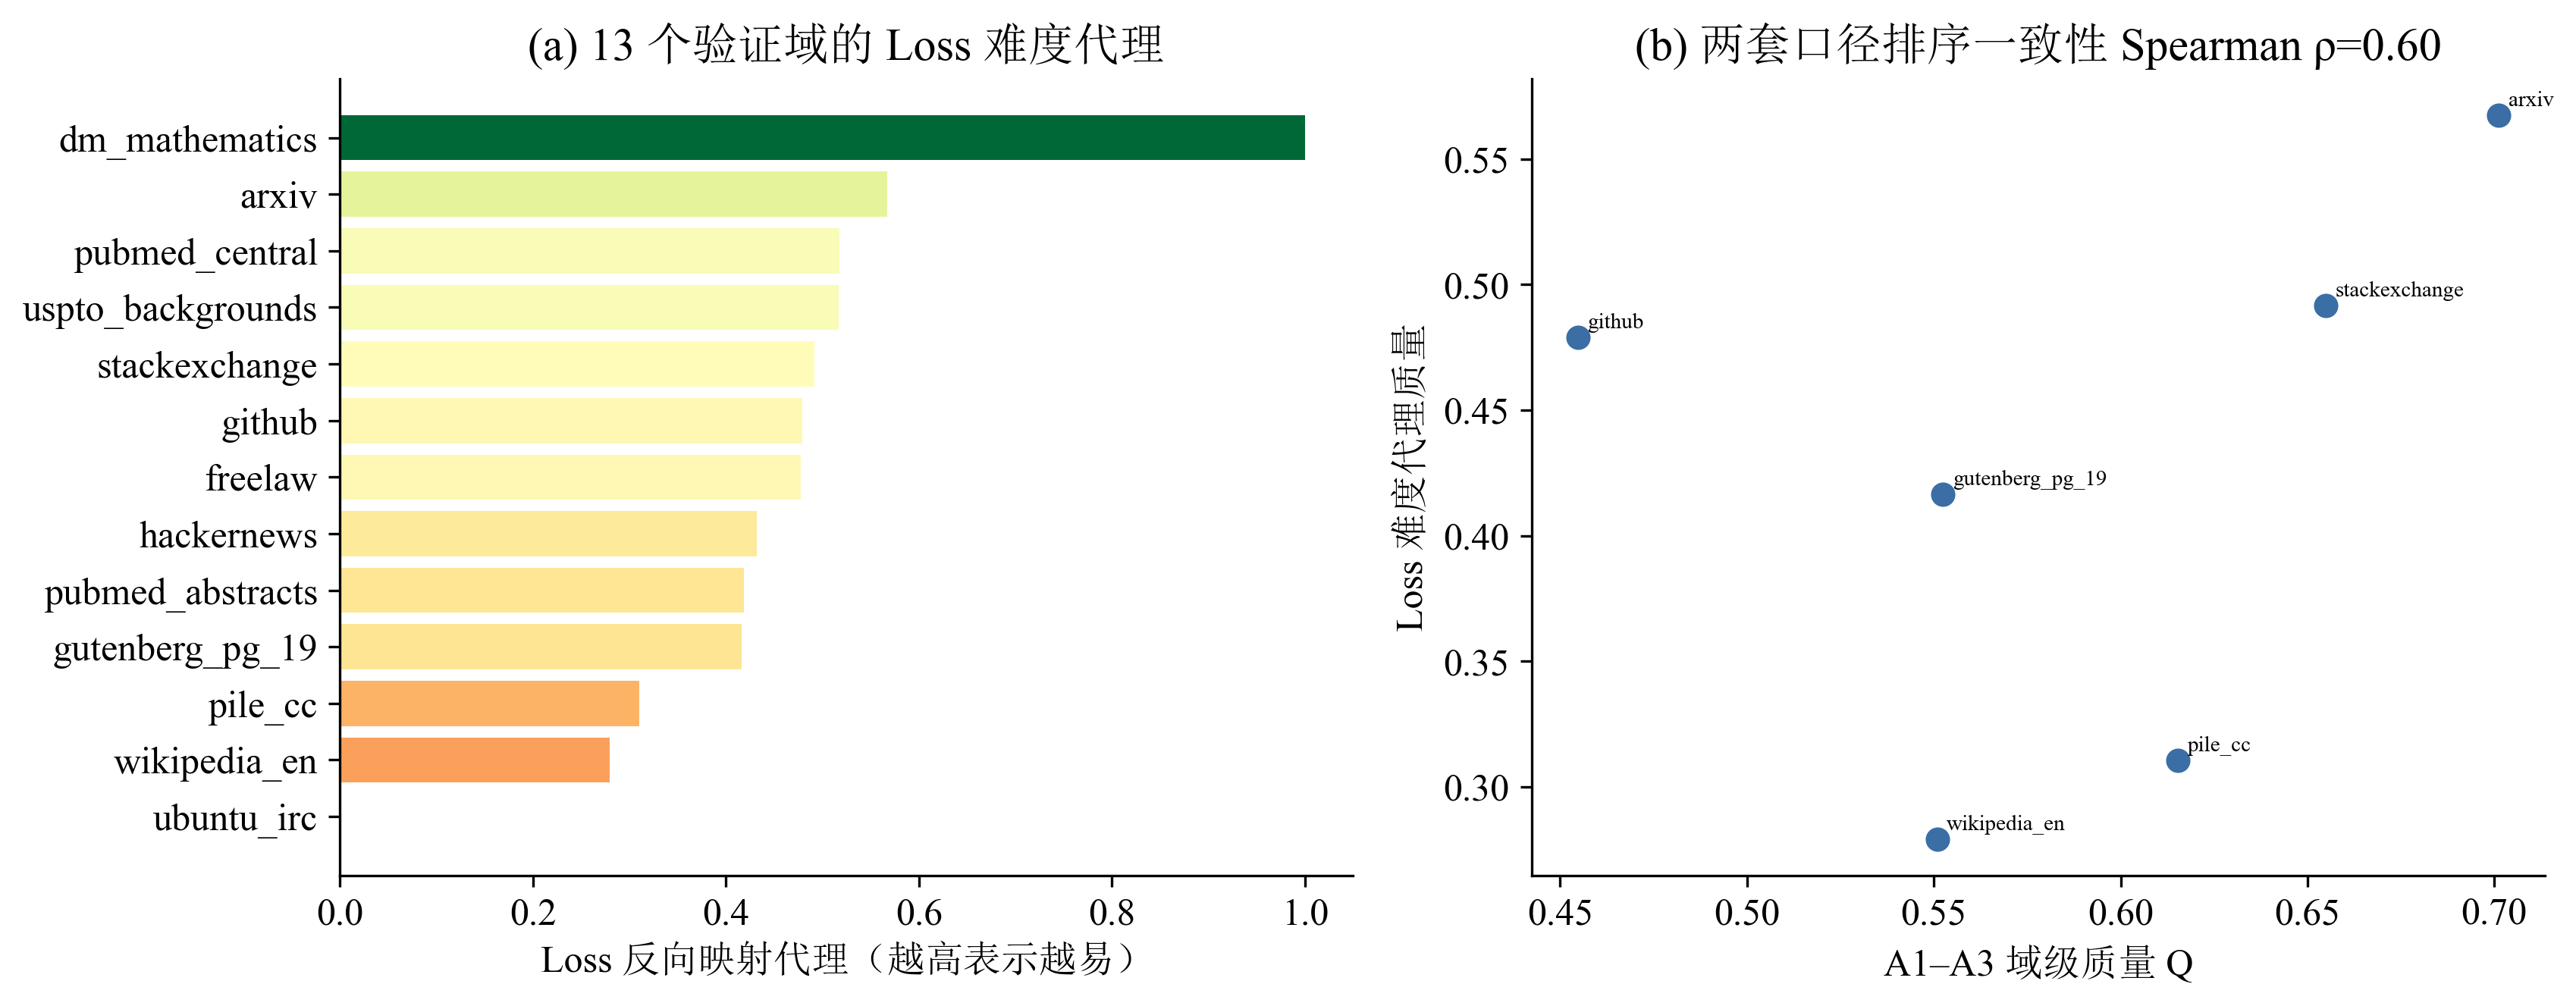
\includegraphics[width=0.92\textwidth]{求解/问题一/图片/图5_领域质量评分.png}
  \caption{左：13 个验证域的损失难度代理；右：A1--A3 质量与损失难度代理的排序一致性}
  \label{fig:p1_quality}
\end{figure}

由图\ref{fig:p1_quality}(a)可知，13 个损失域的内在难度差异显著，dm\_mathematics 最易（代理质量 $1.000$）、ubuntu\_irc 最难（代理质量 $0.000$）；图\ref{fig:p1_quality}(b)显示，A16 的 direct/near\_direct 映射中两套口径的 Spearman 排序相关为 $0.60$：arxiv、stackexchange、github 三个域在两种口径下同向（文本质量高、损失也相对低），但 wikipedia、book、pile\_cc 存在明显分歧——文本质量较高而该域损失并不低（学术与百科长文属“高质量但难拟合”）。因此质量评分必须按用途区分：面向数据治理使用 A1--A3 的文本质量，面向性能预测使用损失难度代理。

\textbf{3.最优配比与跨尺度稳健性}

无约束优化倾向于把配比集中于单一低损失域（预测加权平均损失 $4.177$），不具备可落地性；故采用 2.5 倍上限的有界推荐作为最终方案，推荐配比与参考配比的对比见表\ref{tab:p1_rec}，该方案使预测加权平均损失由 $5.336$ 降至 $5.136$（下降 $0.199$）。

\begin{longtable}{>{\centering\arraybackslash}p{0.30\textwidth}>{\centering\arraybackslash}p{0.22\textwidth}>{\centering\arraybackslash}p{0.22\textwidth}>{\centering\arraybackslash}p{0.20\textwidth}}
  \caption{有界推荐配比调整}
  \label{tab:p1_rec} \\
  \toprule
  领域 & 参考配比 & 推荐配比 & 调整量 \\
  \midrule
  \endfirsthead
  \caption{有界推荐配比调整（续）} \\
  \toprule
  领域 & 参考配比 & 推荐配比 & 调整量 \\
  \midrule
  \endhead
  \bottomrule
  \endfoot
  pubmed\_central & 0.1137 & 0.2843 & $+0.1706$ \\
  stackexchange & 0.0994 & 0.2486 & $+0.1491$ \\
  pubmed\_abstracts & 0.0662 & 0.1654 & $+0.0993$ \\
  gutenberg\_pg\_19 & 0.0469 & 0.1173 & $+0.0704$ \\
  dm\_mathematics & 0.0255 & 0.0637 & $+0.0382$ \\
  uspto\_backgrounds & 0.0755 & 0.0000 & $-0.0755$ \\
  freelaw & 0.0968 & 0.0000 & $-0.0968$ \\
  github & 0.1107 & 0.0000 & $-0.1107$ \\
  arxiv & 0.1130 & 0.0000 & $-0.1130$ \\
  pile\_cc & 0.1195 & 0.0000 & $-0.1195$ \\
\end{longtable}

由表\ref{tab:p1_rec}可知，推荐方案应显著增加 pubmed\_central、stackexchange、pubmed\_abstracts 等学术领域的配比，同时压缩 pile\_cc、arxiv、github、freelaw 等领域的占比。需要说明的是，这一结论是针对“13 个验证域加权平均损失”这一目标的优化结果，与“提升单个域自身表现”并不等价（例如 arxiv 的配比下降并不意味着 arxiv 质量低，而是因为其对加权平均损失的边际贡献为负）。外推稳健性方面，10B 与 70B 外推表的损失尺度因子（est/train）在各损失域上高度一致（10B 均值 $0.338$、标准差 $0.038$；70B 均值 $0.266$、标准差 $0.036$），且同配方下 60M 与 1M 的跨尺度损失比稳定（均值 $0.51\sim0.82$），说明同一套配比—损失系数可在不同参数规模间复用、具备跨尺度外推能力，如图\ref{fig:p1_extrap}所示。

\begin{figure}[ht]
  \centering
  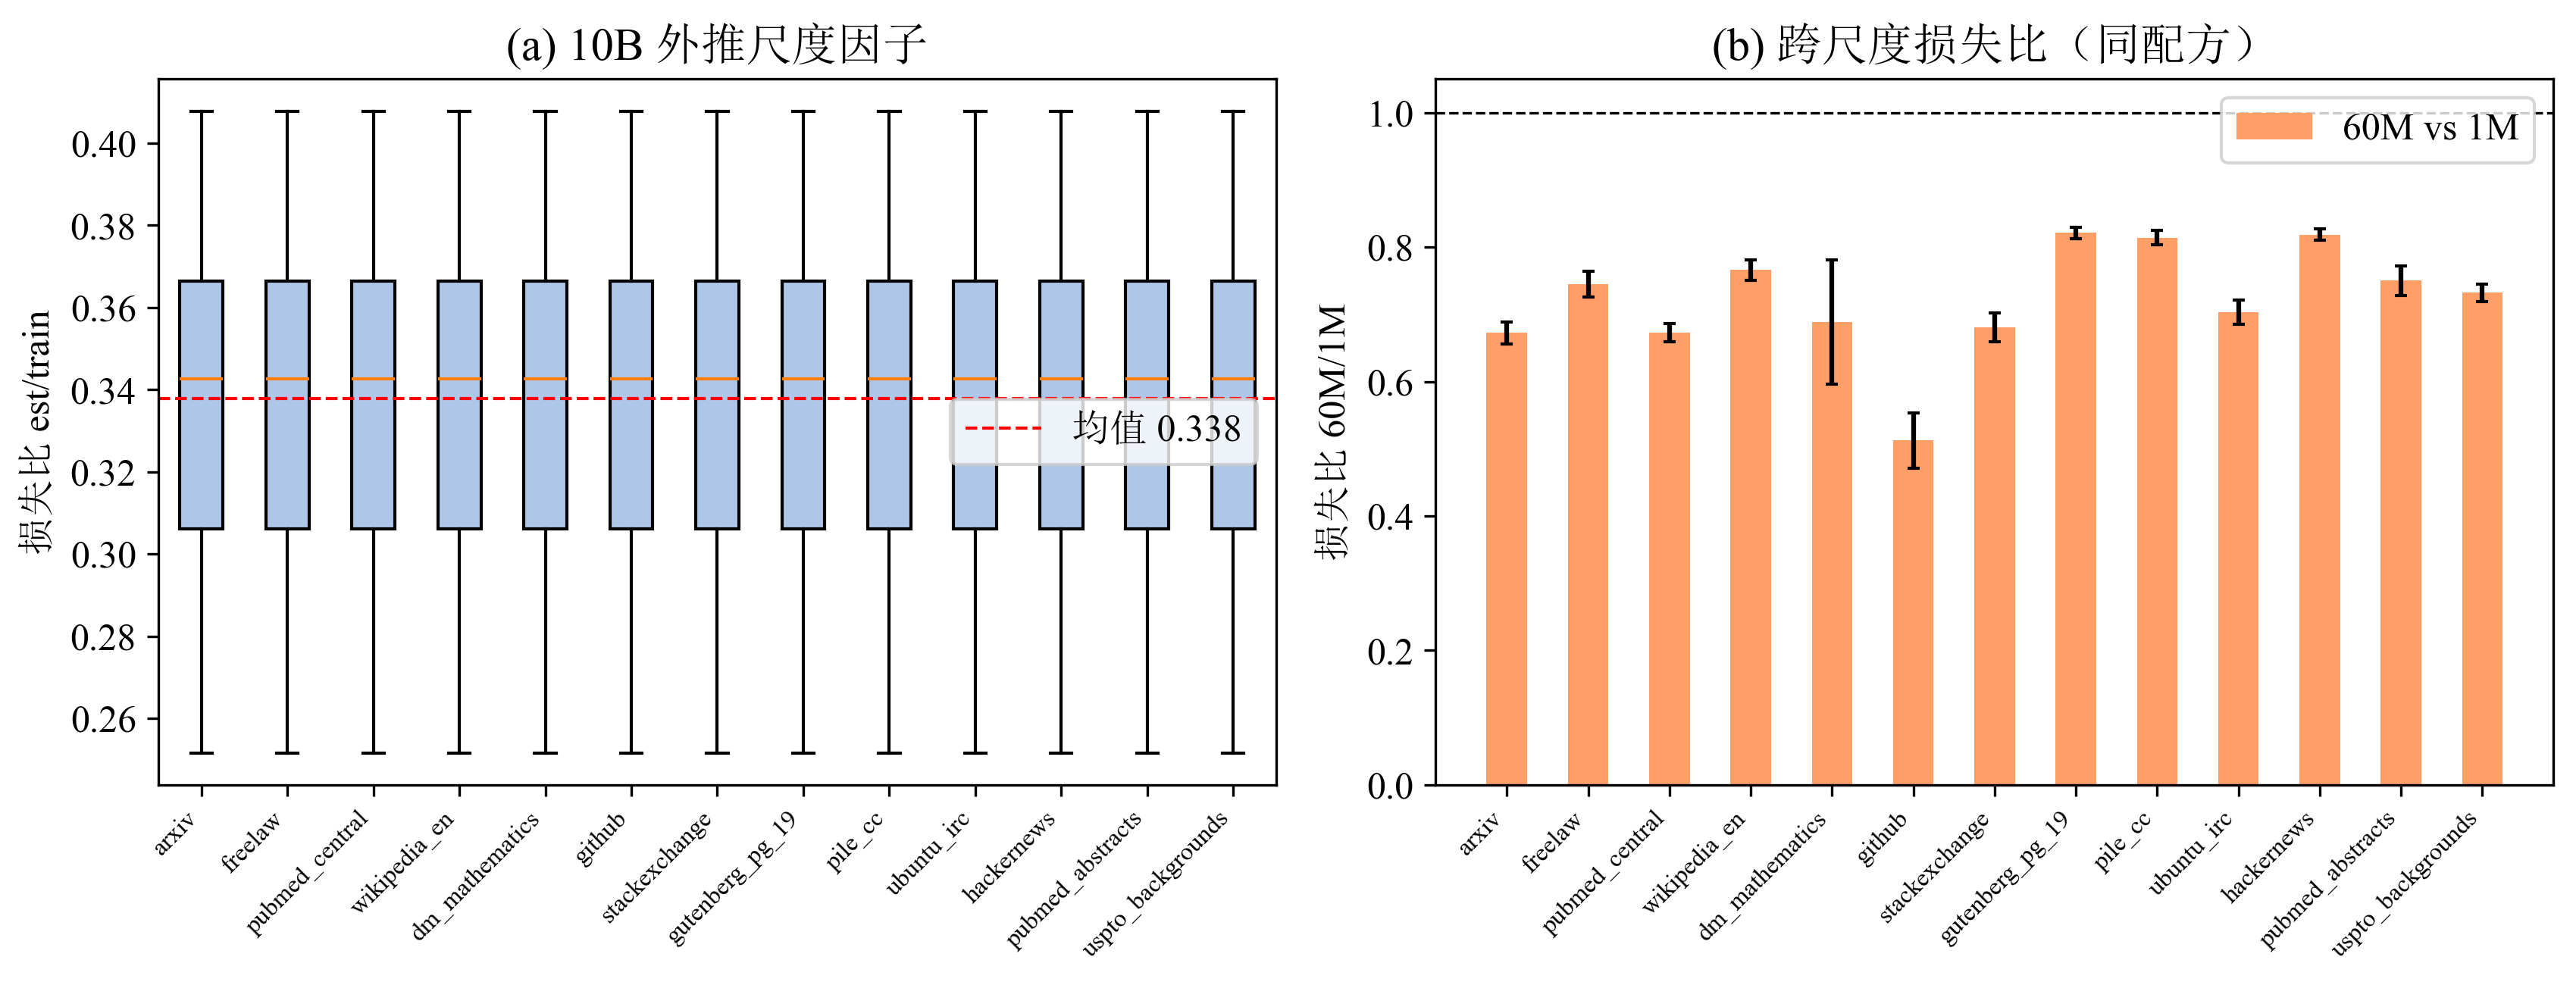
\includegraphics[width=0.92\textwidth]{求解/问题一/图片/图7_外推与跨尺度.png}
  \caption{外推稳健性验证（左：10B 外推尺度因子；右：同配方 60M/1M 跨尺度损失比）}
  \label{fig:p1_extrap}
\end{figure}

综合以上结果，本节完成了问题一的求解，得到领域质量评分 $Q$、最优配比 $\bm p$ 与配比—损失定量关系，为后续问题提供质量与配比输入。
